
\documentclass[english]{cccconf}
\usepackage{amsmath,subfig}
\usepackage{epstopdf}
\usepackage{booktabs }
\usepackage[american]{babel}
%\usepackage{csquotes}
\usepackage{float}
\usepackage{algorithm}
\usepackage{algorithmic}
\usepackage[style=numeric,backend=biber]{biblatex}
\addbibresource{SR.bib}


\begin{document}
	
\title{Heterogeneous Computing for Signal and Data Processing}

\author{E4750\_2017Fall\_SRBISR\_report\\Xiaotong Qiu  xq2174,Yameng Xiao  yx2417,Xiaotian Hu    xh2332\\\textsl{Columbia University}}


\maketitle


\begin{abstract}

Super resolution(SR) is one of the popular image reconstruction technology. One of the approach to it is sparse presentation method. This method learns a low-resolution dictionary and high-resolution dictionary pair to store the high-resolution image. Out team implemented the dictionary learning algorithm for super resolution. We focused on the most time-consuming part of the dictionary-learning algorithm, the K-SVD algorithm and tried to parallel the core part of the K-SVD: Orthogonal Matching Pursuit. The parallelization faced two challenges: the computation scale of the OMP is not fit into a single thread nor a whole GPU. And the memory access in the computation process of OMP is random. We used the batch technology and write series of kernel intended for loading data to solve these two problems. Our program succeeded in getting dictionary that can be used in super resolution. And our parallelization version K-SVD shows a 10 times improvement in speed when compared with sequential version K-SVD. In this report, we discuss the implementation of our program and show some experiment results to show the performance improvement we achieved. 
\end{abstract}


\section{1. Overview}

\subsection{Problem in a Nutshell}
Super resolution(SR)\parencite{jianchao_yang_image_2010,timofte_anchored_2013,kaibing_zhang_multi-scale_2012,nasrollahi_super-resolution:_2014}is a popular image reconstruction problem, it reconstructs the high-resolution image from the low-resolution image. This technology has vast application field including medical imaging, satellite imaging, pattern recognition, etc. 

Dictionary-based method\parencite{jianchao_yang_image_2010,kaibing_zhang_multi-scale_2012} is one of the widely talked method to this problem. It takes a training dataset consists of known low-resolution and high-resolution image pairs and get image patch signals with partition and some successive image processing. Based on this patch signals, it tries to learn a low-resolution dictionary \(A_l\) and high-resolution dictionary \(A_h\) which can represent image patch signals as:
\begin{gather}
    p^h_k = A_hq_k \\
    p^l_k = A_lq_k
	\label{equ1}
\end{gather}

where \(x_l\) and \(x_h\) are the low-resolution and high-resolution image patch signal and \(\alpha\) is the sparse representation. \(\alpha\) is a sparse vector with only a few non-zero elements. \(A_r\) and \(A_l\) are consisted of vectors of the same length of patch signals and these vectors are called atom. Patch signals are actually represented as the linear combination of those atoms and \(\alpha\) is the combination coefficients. Since alpha is sparse\parencite{jianchao_yang_image_2010}, only a few atoms will be used to form the patch signal, hence, the representation alpha is called spares representation. After getting the dictionary pair \(A_r\) and \(A_l\), with the assumption that the corresponding low-resolution patch signal and high-resolution patch signal can be represented as the same sparse representation \(\alpha\) with \(A_r\) and \(A_l\) respectively. The high-resolution image can be reconstructed by computing the spare representation of the low-resolution image patches, mapping their sparse representation, getting the corresponding high-resolution patches and stitching them to get the final output. 

The key step of this method is learning the dictionary pairs \(A_r\) and \(A_l\), one of the algorithm is K-SVD\parencite{aharon_rm_2006}. It iteratively learns the dictionary from the training data. For each iteration, K-SVD firstly compute the spares representation with current dictionary for training signals with some pursuit algorithm and then uses the representation to refine the dictionary to decrease the error of representation. The refining process involves SVD, which gives it the name, K-SVD. In SR problem, K-SVD needs massive computation because the training process usually uses millions of patch signals. 

The computation of K-SVD can be reduced by replacing SVD computation in every step with simple but coarse computation in every iteration.\Cite{irofti_gpu_2014,rubinstein_efficient_2009}. It accelerate the K-SVD method with only a little precision loss. 

Our project focus on parallelizing the key procedure the dictionary learning process: K-SVD. And to achieve better speed performance, the approximated K-SVD\parencite{rubinstein_efficient_2009} is used. And the other part of the dictionary-based super resolution algorithm, which only take a small part of whole computation is implemented in sequential fashion. 

\subsection{Prior Work}
Article \cite{jianchao_yang_image_2010} gives the general framework of dictionary-based approach to the super resolution. And the K-SVD algorithm is detailed described in the article \cite{aharon_rm_2006}. And the article \cite{rubinstein_efficient_2009} comes up with the approximated K-SVD algorithm.


\section{Description}
In this section, we elaborate the details about the implementation of the dictionary learning program. We will first describe the algorithm and then point out the most time-consuming part of the program, the K-SVD, by analyzing the computational complexity. Finally we will discuss in detail about how to parallelize the K-SVD. 
\subsection{Objectives and Technical Challenges}
Implement the parallelized version of dictionary learning algorithm for SR, including 
Two objectives are derived:
\begin{enumerate}
	\item contdesign the dictionary learning program whose routines include extracting patches signals, training the low-resolution dictionary and computing the high-resolution dictionary.
	
	\item parallel the K-SVD part of the dictionary learning program. It involves in parallelizing Orthogonal Matching Pursuit algorithm and handling random memory accessing issues.
\end{enumerate}
 
\subsection{Problem Formulation and Design }
The dictionary learning algorithm tries to find the optimal dictionary pair Al and Ar and sparse representation for training signals that minimize the representation error. It can be formulated as the optimization problem:  
\begin{equation}
	\mathop{\mathrm{argmin}}_{A_l,q_k}\quad\sum_k\big\lVert A_lq_k - h_k^l \big\rVert_2
	\label{equ2}
\end{equation}
\begin{equation}
p_k^h = A_hq_k\quad and \quad \lVert q_k \rVert_0 <<T
\label{equ3}
\end{equation}

Where \(p_k^h\) and \(p_k^l\) is the patch signal from high-resolution images and low-resolution images, and the \(T\) is the sparse coefficients which constrains the largest number of non-elements in the sparse representation \(q_k\)

Dictionary learning routine can be generally divided into 3 steps, which is depicted by flow chart figure~\ref{figh1}
\begin{enumerate}
	\item extract the patch signals from the training images
	\item train the low-resolution dictionary using K-SVD
	\item compute the high-resolution dictionary from the low-resolution dictionary.
\end{enumerate}


\begin{figure}[!htb]
	\centering
	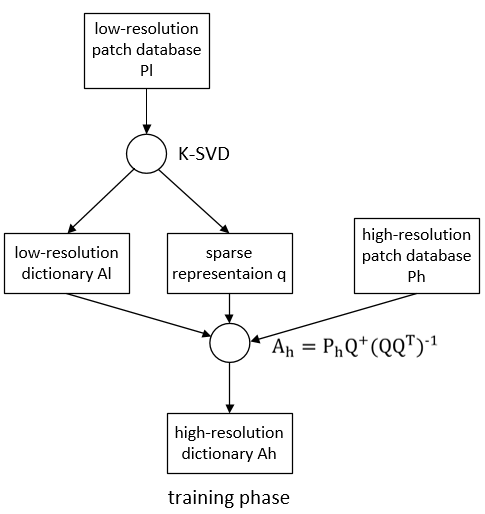
\includegraphics[width=210pt]{2.png}
	\caption{The flow chart of the dictionary learning process. It firstly extract the patches signals, and then learn the low-resolution dictionary. Finally, compute the high-resolution dictionary with a close-form expresssion.}
	\label{figh1}
\end{figure} 


The training process takes around 20 images and extract over 20,000 patch signals for training. This process needs a great amount of computation, most of which is caused by K-SVD. The K-SVD is used to get the low-resolution dictionary, in other word, to solve the sub-problem of problem equation~\ref{equ4} 
\begin{equation}
    \mathop{\mathrm{argmin}}_{A_l,q_k}\quad\sum_k\big\lVert A_lq_k - h_k^l \big\rVert_2
	\label{equ4}
\end{equation}

In each iteration of K-SVD, it computes the sparse representations of all training signals under current dictionary with Orthogonal Matching Pursuit(OMP) algorithm and then use the sparse representation to refine the dictionary. The pseudo code for K-SVD is shown algorithm~\ref{algh1}

\begin{algorithm}[H]
	\caption{Approximate K-SVD} 
	\label{algh1}
	\begin{algorithmic}
		\STATE \textbf{Input}: Singal set \(\mathbf{X}\), initial dictionary \(\mathbf{D_0}\), target sparsity \(K\), number of iterations \(k\)   
		
		\STATE \textbf{Output}: Dictionary \(\mathbf{D}\) and sparse matrix \(\mathbf{\Gamma}\) such that \(\mathbf{X}\approx\mathbf{D\Gamma}\)
		
		\STATE \textbf{Init} Set \(\mathbf{D}\leftarrow\mathbf{D_0}\)
		
		\FOR {\(n=1,\dots,k\)}
		\STATE \(\mathbf{\Gamma}=\mathrm{OMP}(\mathbf{X},\mathbf{D})\)
		\FOR {\(j=1,\dots,L\)}
		\STATE \(\mathbf{D}_j\leftarrow0\)
		\STATE \(I\leftarrow\)\{ \textsl{indices of the signals in \(\mathbf{\Gamma}_i\) whose \(i\) element is non-zero}  \}
		\STATE \(g\leftarrow\mathbf{\Gamma}^T_{j,I}\)
		\STATE \(d \leftarrow \mathbf{X}_{I}g - \mathbf{D\Gamma}_{I}g\)
		\STATE \(d \leftarrow d/\lVert d\rVert_2\)
		\STATE \(g \leftarrow \mathbf{X}_I^Td-(\mathbf{D\Gamma_I}^T)d\)
		\STATE \(\mathbf{D}_j \leftarrow d  \)
		\STATE \(\mathbf{\Gamma}_{j,I} \leftarrow g^T \)
		\ENDFOR
		\ENDFOR
	\end{algorithmic}
\end{algorithm}

The main cause of the great amount of computation of K-SVD is that it will perform over 10,000 OMP in each iteration. Hence, the acceleration of  the OMP procedure is the key to accelerate the entire K-SVD algorithm. In the next paragraph, the computation complexity of OMP will be analyzed in detail. 

\begin{algorithm}[H]
	\caption{Orthogonal Matching Pursuit(OMP)} 
	\label{algh2}
	\begin{algorithmic}
		\STATE \textbf{Input}: Dictionary \(\mathbf{D_0}\), batch of signals \(X = \{x_i\}\), target sparsity \(T\)   
		
		\STATE \textbf{Output}: Sparse Representations \(\Gamma\) 
		
		\STATE \textbf{Init} Set \(I\leftarrow\{\},\,R\leftarrow X,\Gamma\leftarrow0\)
		
		\FOR {\(i=1,\dots,T\)}
		\STATE \(\mathbf{K}\leftarrow \mathbf{D}R \)
		\STATE \(k^* \leftarrow \max{\{\mathbf{K}\}}\)
		\STATE \(I \leftarrow (I,k^*)\)
		\STATE in batch solve \(x_i = \mathbf{D}_Ir_i\)
		\STATE in batch compute \(r_i\leftarrow x_i - \mathbf{D}_I\gamma_I\) where \(R = {r_i}\)
		\ENDFOR
	\end{algorithmic}
\end{algorithm}

Algorithm~\ref{algh2} is the pseudo code of OMP algorithm. The operations of iteration include computing serval times of inner products, solving a overcomplete linear system and performing a matrix multiplication and subtraction. For a typical super resolution problem, low-resolution is consisted of over 1000 atoms and the size of each atom vector is around 50. Besides, each sparse representation will contain less than 5 non-zeros elements. Hence, for each iteration of OMP, there are over 1000 inner products, a linear system with size of \(30 \times 5\) and matrix multiplication and subtraction with matrices size of \(30 \times 5\) matrices in total.

The scale of computation for OMP brings a challenge: it is too large to fit into a single CUDA thread, is also not large enough to use a CUDA grid to compute, which will cause a great waste of GPU resources. Therefore, the batch technology is used. With batch, GPU resource can be shared by more than one streaming each of which computes a linear system solver or matrix multiplication for one signal OMP operation.  

Besides the resource allocation, the memory access pattern of OMP operation also raises a challenge. For each iteration of single OMP, the program loads the dictionary atom corresponding to the largest inner product, which means which atoms to be loaded is not determined until the run time, depicted by figure~\ref{figh2}

\begin{figure}[!htb]
	\centering
	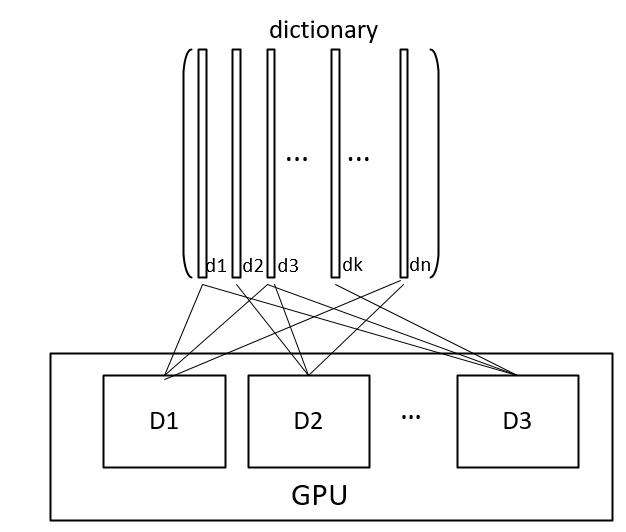
\includegraphics[width=210pt]{3.png}
	\caption{The memory access pattern of OMP. The dictionary atoms will be loaded into device and which atoms will be loaded is not determined until the running time.}
	\label{figh2}
\end{figure} 

The atom selecting and loading tasks are executed by CPU with cudaMemcpy function in traditional way. It will cause a great number of memory access between host and device, which is an intolerably time-consuming. To mitigate the impact of random memory access, we write series of dedicated GPU kernel programs to do the atom loading. 

\subsection{Software Design}

To make the report concise, the pseudo code for the whole dictionary learning program is placed in the appendix.A, and we focus the parallel part of our code in this section. The algorithm~\ref{algh1} describes K-SVD and the algorithm~\ref{algh3} shows the parallelized version OMP.

\begin{algorithm}[H]
	\caption{Parallelized Orthogonal Matching Pursuit(OMP)} 
	\label{algh3}
	\begin{algorithmic}
		\STATE \textbf{Input}: Dictionary \(\mathbf{D_0}\), batch of signals \(X = \{x_i\}\), target sparsity \(T\)   
		
		\STATE \textbf{Output}: Sparse Representations \(\Gamma\) 
		
		\STATE \textbf{Init} Set \(I\leftarrow\{\},\,R\leftarrow X,\Gamma\leftarrow0\)
		
		\FOR {\(i=1,\dots,T\)}
		\STATE \(\mathbf{K}\leftarrow \mathbf{D}R \)
		\STATE \(k^* \leftarrow \max{\{\mathbf{K}\}}\)
		\STATE \(I \leftarrow (I,k^*)\)
		\STATE in batch solve \(x_i = \mathbf{D}_Ir_i\)
		\STATE in batch compute \(r_i\leftarrow x_i - \mathbf{D}_I\gamma_I\) where \(R = {r_i}\)
		\ENDFOR
	\end{algorithmic}
\end{algorithm}

The parallelized OMP processes one batch of signals for each run. It has 5 steps for each iteration. We will discuss the implementation details of these 5 steps respectively.

The first step is to compute the inner products between the dictionary atoms and the signal vectors. This operation can be realized with a single matrix multiplication as shown in the pseudo code, where \(\mathbf{X}\) is the combination of batch signals whoes column corresponding to those patch signal.

The second and third steps are to find the position of the atom with the max inner production and assign the found indices into the atom loading pointer \(I\). These two steps are implemented within a kernel program, which find the max element of each column of input matrix and set the corresponding element to 1 in the output matrix.

Step 4 solves linear system for each signal in batching fashion. Before performing the computation, the corresponding matrix \(\mathbf{D}_I\) and \(x_i\) should be loaded into device according to the atom loading pointer \(I\). 


Step 5 calculates the current residues for each signal between its representation and itself, and, the same as the fourth step, it also should load the related data into device.

We write the dedicated kernel to do the data loading job for step 4 and step 5, and use the cuBlas API to solve the linear system.

At the end of the OMP iteration, the output should be converted from dense format into sparse format. Another kernel has been written to perform this conversion.

\section{Results}
\subsection{Dictionary Learning Algorithm Result}
In our project, we firstly implemented the pure python version of dictionary learning algorithm. It takes 20 images as training dataset and output a dictionary with 1024 atoms each of which is a vector of size 30. The dictionary can used to restore the high -resolution images, shown as the following figure~\ref{figh3}
\begin{figure}[!htb]
	\centering
	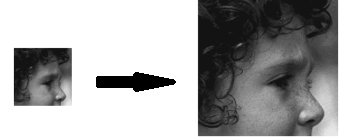
\includegraphics[width=210pt]{7.png}
	\caption{The high-resolution image is successfully restores from low-resolution image with our dictionary}
	\label{figh3}
\end{figure} 

\subsection{Performace Comparison of K-SVD}
We tested our parallelized K-SVD algorithm on the tesseract server. This server equipped an 8-cores 8 Intel(R) Xeon(R) CPU of clock frequency 1.8GHz, and Tesla k40c GPU. We feed the K-SVD program with the data extracted from out dictionary learning program. In the testing scenario, the K-SVD takes 8172 patches  signals vector of size 30 and output a dictionary of size \(30\times1024\). It takes the CPU version program 63.044 seconds while takes GPU version only 6.664 seconds, which means the parallelization brings around 10 times performance improvement in speed.

\subsection{impact of batching and dedicated kernel}
During our programming work, the first version of parallelized OMP did not use the batch technology and dedicated data loading kernel. This program used CPU to select the atom to load and transferred the atom from CPU to GPU. It achieves a poor performance with only 2 times improvement in speed. The nvvp analyze result for the program is shown below in figure~\ref{figh4}

\begin{figure*}[!htb]
	\centering
	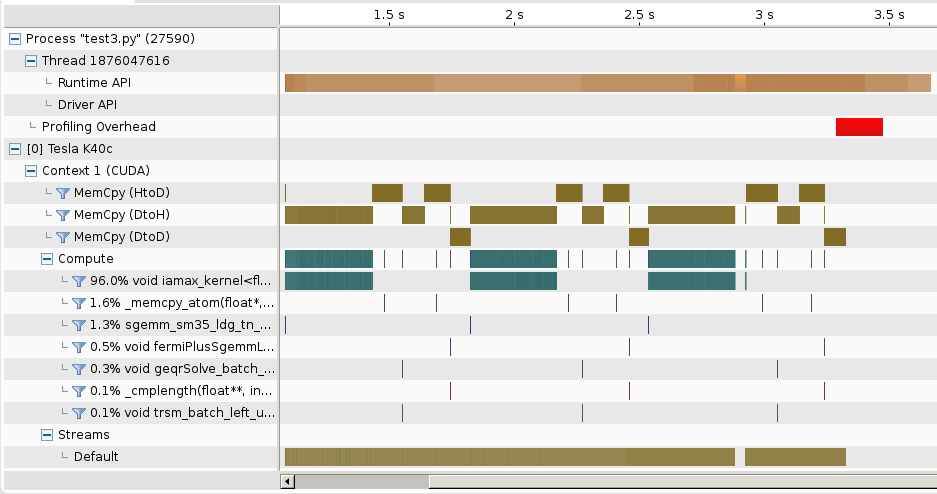
\includegraphics[width=450pt]{4.png}
	\caption{The nvvp analysis of the naive parallelized OMP}
	\label{figh4}
\end{figure*} 

It can be observed the running time of this program is divided into 3 segments which corresponds to 3 iteration. The memory copy from host to device and from device to host takes the most time of computation, which means the frequent memory interaction between the host and device lowered the program speed to a great extent.

Beside the cudaMemcpy API, the imax\_kernel took the second largest portion of the program running times. This kernel was used to find the atom corresponding the max inner product for every signal. It needs to be ran thousands of times in  each iteration in our case, and, even worse, it needs call cudaMemcpy API for each run. 

This program was modified with batching and dedicated kernel. We write a new kernel to find the maximum for all signal simultaneously and designed series of kernel to move data between different bucks of device memory. The performance of the program dramatically changed after the modification. It achieves around 180 times of improvement in speed when compared with the CPU version OMP. The nvvp analysis is shown in below figure~\ref{figh5}

\begin{figure*}[!htb]
	\centering
	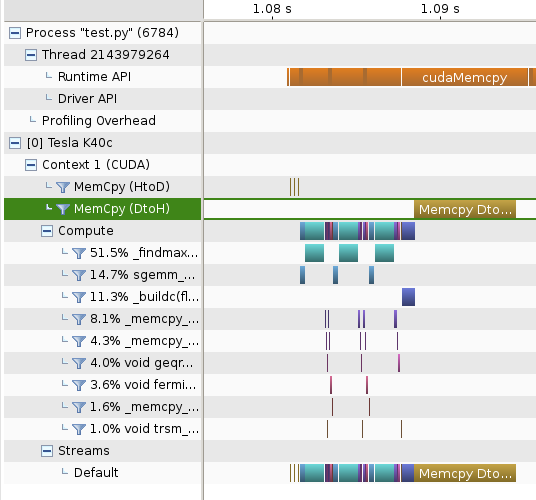
\includegraphics[width=400pt]{5.png}
	\caption{The nvvp analysis of the imporved parallelized OMP}
	\label{figh5}
\end{figure*} 

It can be seen that with those new kernels, all computations are performed on the GPU and therefore no data interaction between device and host happens during the iterations. The maximum finder kernel costs much less computation time and is not the bottleneck of the speed anymore. 

In conclusion, by using batching kernel and dedicated data loading kernel and put all computation onto the GPU, the parallelized program achieves a significant speed acceleration. 

\section{Discussion and Further Work}
We succeed in parallelizing the K-SVD and achieve an around 10 times improvement in speed. However, this program can be further optimized with respect of speed. On the one hand, besides the OMP part of K-SVD, the atom refinement phase can also be parallelized. It has the similar operation like OMP and can also be speeded up with batching technology and dedicated kernel for loading. On the other hand, there exists parallelized code outside the K-SVD in the dictionary learning program including principle component analysis(PCA) process in the patch- signal- extracting routine.
\section{Conclusion}
In our project, we succeed in implementing the dictionary learning algorithm and parallelizing the core of this algorithm – K-SVD. With the parallelized version of K-SVD, the speed of the dictionary training process was improved to a large extent. To parallelize the K-SVD, we learned the batching technology that can make GPU run several kernels simultaneously. After implementing and comparing the performance of parallel version programs implemented with cudaMemcpy function and dedicated  kernel respectively, we noticed the memory access between host and device is usually the most time-consuming part of the whole program. To achieve better performance, the CUDA program should avoid the data interaction between host and device. 
 
Although our work has improved the speed of dictionary training algorithm, there exists other processes in the whole program which can be parallelized to achieve further improvement such as the principle component analysis in the patch- signal- extraction phase. 



\section{Appendix.A}
The pseudo code for the overall dictionary learning

	\begin{algorithm}[H]
		\caption{Dictionary-Learning Process} 
		\label{alg1}
		\begin{algorithmic}
			\STATE \textbf{STEP  1.} Load training images.
			
			\STATE \textbf{STEP  2.} Converts images from RGB color space to YCbCr color space and save the illuminance(Y) value.
			
			\STATE \textbf{STEP  3.} Crop the images and save as \textbf{high resolution images} set.
			
			\STATE \textbf{STEP  4.} Downsampling the high resolution images to get \textbf{low resolution images} set.
			
			\STATE \textbf{STEP  5.} Upsampling the low resolution images to get \textbf{middle resolution images} set.
			
			\STATE \textbf{STEP  6.} Call \textit{collect} function to extract features for each image in middle resolution set and get \textbf{features} matrix.
			
			\STATE \textbf{STEP  7.} Upsampling the low resolution images to get  \textbf{interpolated images} set.
			
			\STATE \textbf{STEP  8.} Subtract each images in high resolution set and in interpolated images set to get patches set.
			
			\STATE \textbf{STEP  9.} Call \textit{collect} function to extract features for each image in patches set and get \textbf{patches} matrix.
			
			\STATE \textbf{STEP 10.} Implement dimensionality reduction on features matrix based on PCA and get \textbf{features\_pca} matrix.
			
			\STATE \textbf{STEP 11.} Call \textit{ksvd} function using features\_pca to train for the \textbf{low resolution dictionary} as well as \textbf{gamma} matrix.
			
			\STATE \textbf{STEP 12.} Calculate high resolution dictionary $D_h$ using formula : $D_h = PQ^T(QQ^T)^{-1}$  (P: patches matrix  Q: gamma matrix)
			
		\end{algorithmic}
	\end{algorithm}

\printbibliography
\end{document}






